\documentclass[../main.tex]{subfiles}
\begin{document}

\chapter{Lecture 19 - 18-05-2020}

$$
k(x,x') = < \phi(x), \phi(x')>
\qquad \phi: X \rightarrow H
$$
where $X \rightarrow \barra{R}^2$ and $H \rightarrow barra{R}^N $
$$
H_\delta = \{ \sum_{i =1}^N \alpha_i \, k_\delta (x_i, \cdot), x_1,..., x_N \in \barra{R}^d, \alpha_1, ... \alpha_N, N \in \barra{N } \} 
$$
Inner product measures "similarities" between data points.
\\
$$
x^T \, x' = \|x\| \, \|x'\| \, \cos \Theta \qquad x \in X \quad k(x,x')
$$
$k$ sais how much similar are the structure (tree, documents etc).
\\
I would like to learn a predictor based on the notion of similarity.
\\
$$
k(x,x') = < \phi(x), \phi(x')>
$$
where $<>$ is the inner product.
\\
So we have Data $\rightarrow$ Kernel $\rightarrow$ Kernel learning Algortithm
\\
Kernels offer a uniform interface to data in such way they algoriithm can learn from data.
\\
Given $K$ on $X$, I need to find $\exists H_k \quad \phi_k \ X \rightarrow H_k$
\\
$\exists <...>_k$ s.t $k(x,x') = <\phi_k(x), \phi_k(x')>_k $
\\\\
\bred{Theorem}
\\
Given $K: X \times X \rightarrow \barra{R}$, symmetric
\\
Then $K$ is a Kernel iif $\forall m \in \barra{N}$ $\forall x_1,...,x_m \in X$
\\
The $m \times m$ matrix $K$ \quad $K_{ij} = k (x_i,x_j)$ is positive semidefinite\\
$
\forall \alpha \in \barra{R}^m \qquad \alpha^T \, K \, \alpha \geq 0
$ 
\\
In general, given a Kernel $K$ there is not unique representation for $\phi_k$ and $<...>_k$ (inner product).
\\
However,  there is a "canonical" representation: 
$
\phi_k(x) = K(x, \cdot)
$
$$
\phi_k : X \rightarrow H \qquad H_k = \{ \sum_{i=1}^N \alpha_i \, k (x_i, \cdot ), \alpha_1,..., \alpha_N \in \barra{R}, x_1,...,x_N \in X, N \in \barra{N} \}
$$
We have to define an inner product like:
$$
<\phi_k(x), \phi_k(x')>_k \ = \ k(x,x')
$$
This is the canonical representation that helps mapping.
\\\\
What happen to use this mechanism to perform predictions?
\\
$
x \in \barra{R}^d \ w \in \barra{R}^d \ w^T \, x \qquad \textit{\ where } g = \sum_{i=1}^N \alpha_i \, k (x_i, \cdot)
$
$$
\phi_k(x) \qquad g \in H_k \qquad <g, \phi_k(x)>_k \ = \ <\sum_i \alpha_i k(x_i, \cdot), \phi_k(x)> \  = $$
We have to satisfy allinearity
$$
= \ \sum_i \alpha_i <k(x_i, \cdot), k(x, \cdot) >_k \ = \ \sum_i \alpha_i <\phi(x_i), \phi_k(x)>_k \ = \ \sum_i \alpha_i k(x_i, x) = g(x)
$$
At the end we have:
$$
<g, \phi_k(x)>_k \ = \ g(x)
$$
\\\\
Now, if i have two functions:
$$
f = \sum_{i=1}^N \alpha_i \, k(x_i, \cdot) \qquad g = \sum_{j=1}^M \beta_j \, k (x'_j, \cdot) \qquad f,g \in H_k
$$
$$
<f,g>_k = <\sum_i \alpha_i \, k(x_i,\cdot) , \sum_j \beta_j \, k(x'_j, \cdot) >_k \ =
\ \sum_i \sum_j \alpha_i \, \beta_j <k(x_i, \cdot), k(x'_j, \cdot>_k \ =
$$
$$
= \ \sum_i \sum_j \alpha_i \, \beta_j \, k(x_i, x_j)
$$
$$
\|f\|^2 = <f,f>_k = \sum_{ij} \alpha_i \, \alpha_j \, k(x_i, x_j)
$$
Perceptron convergence theorem in kernel space:
$$
M \leq \|U\|^2 ( \max_t \|x_t\| ^2) \qquad \forall u \in \barra{R}^d \quad y_t \, u^T \, x_t \geq 1 quad \forall g \in H_k \quad y_t \, g(x_t) \geq 1
$$
we know that:
$$
\|x_t \|^2 \rightsquigarrow \| \phi_k(x_t)\|^2_k \ = \ <\phi_k(x_t), \phi_k(\alpha_t) >_k \  = \ k (x_t,x_t)
$$
so 
\\
.... MANCA ULTIMA FORUMA
\\\\
Ridge regression:
$$
w = \left( \alpha \, I + S^T \, S \right)^{-1} \, S^T \, y
$$
$S$ is $m \times d$ matrix whose rows are the training points $x_1,..., x_m \in \barra{R}^d$
\\
$y = (y_1,...,y_m) \quad y_t \in \barra{R}^d$ training labels $\alpha >0$
$$
\left( \alpha \, I + S^T \, S \right)^{-1} \, S^T \ = \ S^T \left( \alpha \, I_m + S\, S^T\right)^{-1}
$$
where $d \times d$ and $d \times m $ = $ d \times
m$ and $m \times m$
$$
\left( S \, S^T\right)_{ij} = x_i^T x_j \qquad \rightsquigarrow \ <\phi(x_i),\phi(x_j)>_k = k(x_i, x_j) = K_{ij}
$$ 
$$
S^T = \left[ x_1,...,x_m \right] \ \rightsquigarrow\ \left[  \ \phi_k(x_i),..., \phi_k(x_m) \ \right] = \left[ \ k(x_1, \cdot), ..., k(k_m, \cdot) \  \right] \ = \ k(\cdot)
$$ 
$$
k (\cdot)^T \, \left( \alpha \, I_m + K \right)^{-1} \, y \ = \ g
$$
where $1 \times
m$ and $m \times
m$ and $m \times
1$\\\\
How to compute prediction?
$$
g(x) = y^T \left( \alpha \, I_m + K \right)^{-1} \, k(x) 
$$
\qquad $1 \times m$ and $m \times m$ and $m \times 1$
\\
In fact, is the evaltuation of $g$ in any point $x$.
\\
The drawback is that we pass from $d \times d$ matrix to a $m \times m$ matrix that can be huge. So it is not really efficient in this way, we need to use addictional "tricks" having a more compact representation of the last matrix prediction. 
\newpage
\section{Support Vector Machine (SVM)}
It is a linear predictor and is a very popular one because has better performance than perceptron and we will see it for classification but there are also version for regression.
\\\\
The idea here is that you want to come up with an hyperplane that is defined as a solution of an optimisation problem.
\\
We have a classification dataset $(x_1,y_1)...(x_m,y_m) \qquad x_t \in \barra{R}^d \quad y_t \in \{ -1,1 \}$ and it is linearly separable.
\\
Sum as the solution $w^*$ (optimisation problem) to this problem:
$$
\min_{w \in \barra{R}^d} \frac{1}{2} \| w \|^2 \qquad s.t \quad y_t \, w^T \, x_t \geq 1 \quad t = 1,2,...,m
$$
Geometrically $w^*$ corresponds to the maximum marging separating hyperplane like:
$$
\gamma^* = \max_{u: \|u\|=1} y_t \, u^t \, x_t \qquad t=1,...,m
$$\
\textbf{$u^*$ is achieving $\gamma^*$ is the maximal margin separator.}\\
\begin{figure}[h]
    \centering
    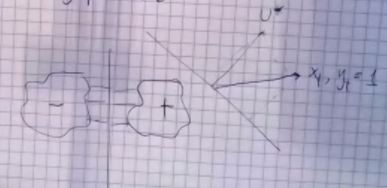
\includegraphics[width=0.4\linewidth]{../img/lez19-img1.JPG}
    \caption{Draw of SVG}
    %\label{fig:}
\end{figure}\\
So I want to maximise this distance.
$$
\max_{\gamma > 0} \, \gamma^2 \qquad s.t \quad \| u \|^2 = 1 \qquad y_t \, u^t \, x_t \geq \gamma \quad t=1,...,m
$$
So we can maximise instead of minimising.
\\
What is the theorem? The equivalent between this two.
\\\\
\bred{Theorem}:\\
$\forall$ linear separator $(x_1,y_1)...(x_m,y_m)$ \\
The max margin separator $u^*$ satisfies $u^* = \gamma^* \, w^*$ where $w^*$ is the SVM solution and $\gamma^*$ is the maximum margin.
\end{document}